%%%%%%%%%%%%%%%%%%%%%%%%%%%%%%%%%%%%%%%%%
% University/School Laboratory Report
% LaTeX Template
% Version 3.1 (25/3/14)
%
% This template has been downloaded from:
% http://www.LaTeXTemplates.com
%
% Original author:
% Linux and Unix Users Group at Virginia Tech Wiki 
% (https://vtluug.org/wiki/Example_LaTeX_chem_lab_report)
%
% License:
% CC BY-NC-SA 3.0 (http://creativecommons.org/licenses/by-nc-sa/3.0/)
%
%%%%%%%%%%%%%%%%%%%%%%%%%%%%%%%%%%%%%%%%%

%----------------------------------------------------------------------------------------
%	PACKAGES AND DOCUMENT CONFIGURATIONS
%----------------------------------------------------------------------------------------

\documentclass{article}

\usepackage{graphicx} % Required for the inclusion of images
\usepackage{natbib} % Required to change bibliography style to APA
\usepackage{amsmath} % Required for some math elements 
\usepackage{amsthm}
\usepackage[hyphens]{url}
\usepackage{hyperref}
\usepackage{subcaption}
\usepackage{float}
\usepackage{array}
\usepackage{amssymb}
\usepackage{tikz}
\usetikzlibrary{backgrounds,calc,shadings,shapes.arrows,shapes.symbols,shadows}
\usepackage{listings}

\setlength\parindent{0pt} % Removes all indentation from paragraphs

\newtheorem*{remark}{Theorem}
\newtheorem*{definition}{Definition}

%----------------------------------------------------------------------------------------
%	DOCUMENT INFORMATION
%----------------------------------------------------------------------------------------

\title{Homework \#6 \\Message Exchange Protocol Design \\[0.2em]\small{}CNS Course Sapienza} % Title and subtitle

\author{Riccardo \textsc{Prinzivalle}, 1904064} % Author name

\date{December 11, 2020} % Date for the report

\begin{document}

\maketitle % Insert the title, author and date

%----------------------------------------------------------------------------------------
%	SECTION 0
%----------------------------------------------------------------------------------------

\section{Homework Goal}

This homework contains a basic design and implementation of a message exchange \textit{secure} protocol. The idea is taken from different protocols learned from the slides and the lessons of the course. The implementation is done using the \textbf{Kathara} framework to virtualize a small network, while the protocol is written using bash scripting exploiting the \textbf{OpenSSL} library on Linux.

%----------------------------------------------------------------------------------------
%	SECTION 1
%----------------------------------------------------------------------------------------

\section{Protocol Design}

The protocol can be divided into three main functionalities: \textit{confidentiality}, \textit{message authentication} and \textit{entity authentication}. Each functionality is developed as follows:

\begin{itemize}
	\item \textbf{Confidentiality} is achieved by using symmetric encryption with AES in CBC mode with key length of 256 bits, which is the standard for confidentiality for NSA \cite{AES_NSA}, similar hint was found also here \cite{AES_stack}.
	\item \textbf{Message Authentication} is performed with SHA-256 using public key signature (OpenSSL supports directly HMAC but the version installed on the docker image on the background of Kathara is older than the minimum version implementing HMAC).
	\item \textbf{Entity Authentication} is based on a weaker version of the X.509 protocol, which introduces some vulnerabilities but simplifies the implementation, since this part is done by hand since OpenSSL contains only the primitives and not a complete authentication protocol. 
\end{itemize}

Let's analyze every part more in the details; weaknesses will be analyzed in section \ref{sec:secAn}.\newline
Encryption is the simpler; it is just based upon the primitive from OpenSSL, and it uses the primitive as follows: 

\begin{lstlisting}[breaklines]
	openssl aes-256-cbc -in message/to/encrypt -out encrypted/message.enc -pass file:key/file
\end{lstlisting}

The key used is based on a shared secret from a DH key exchange phase performed previously, and the instructions needed and used in this work can be found in \cite{DHKE}. The secret is then hashed in order to obtain the desired length of 256 bits for the encryption key. The instruction used is:

\begin{lstlisting}[breaklines]
	openssl dgst -sha256 -out hashed/key.sha256 shared/secret.bin
\end{lstlisting}

To decrypt the message, it is easy as the encryption, it is just necessary to have the shared secret, derive the key by using hashing (as seen upside) and then decrypt with the following command:

\begin{lstlisting}[breaklines]
	openssl aes-256-cbc -d -in encrypted/message.enc -out decrypted/message -pass file:key/file
\end{lstlisting}

As already said, OpenSSL implements different primitives for authenticating messages, the problem resides in the version shipped with the docker image used in the practical experiment: it is older, so it does not support these new addition to the library. Due to this inconvenience, I found \cite{signatures} that it is possible to use message digest with SHA256 with a public key pair for digital signature of a message using OpenSSL, the command is the following:

\begin{lstlisting}[breaklines]
	openssl dgst -sha256 -sign private/key.pem -out message/signature.sha256 encrypted/message.enc
\end{lstlisting}

Then both the encrypted message and its signature are sent to the recipient of the message. \newline
The most complicated part is the entity authentication: the idea is taken from the X.509 protocol, with the idea to simplify it and, in an undesired way, weaken it, this is due to the lack of time to build the protocol from scratch. This part is based on a fusion of \cite{certificates1} and \cite{certificates2}. An entity starting a message exchange must verify its interlocutor and can optionally ask to its interlocutor to verify its identity (sender identity). To perform entity authentication we must define a third party entity, which both the interlocutors trust, which can guarantee the identity of interlocutors on the net: this new entity is called \textbf{Certificate Authority (CA)}. First of all, to define a CA it is necessary to define a master key, as follows: 

\begin{lstlisting}[breaklines]
	openssl genrsa -aes256 -out CA_key.private -passout pass:password 4096
\end{lstlisting}

The key is generated with RSA of length 4096 bits and then encrypted with AES @ 256 bits. It is useful to use a large number of bits for this key since most of the security of the authentication resides on it, we are going to generate a root CA so it is necessary to adopt all security precautions that are possibles. Once a master key for the CA is created, it is possible generate a root certificate for the CA: in real world implementations, it is used a chain of trusted CA, and the root CA are only few and "bulletproof", and there exists a hierarchy of CA; in this case we'll use a single CA that acts as root. To generate the root certificate, it is used the following instruction:  

\begin{lstlisting}[breaklines]
	openssl req -x509 -new -nodes -key CA_key.private -sha256 -days 1825 -out CA_root.pem -passin pass:password
\end{lstlisting}

The password is needed to decrypt the private key which was previously encrypted; then it is necessary to specify the number of days of validity for the certificate. We must keep this certificate under high security layers, since as for the master key, the trust of entity authentication is based on this certificate. Once the root certificate is generated, then the CA can start signing certificates for entities who asked for: the entity asked signing by sending a \textbf{Certificate Signing Request (CSR)} that the CA can use to generate the related certificate:

\begin{lstlisting}[breaklines]
	openssl x509 -req -in user.csr -CA CA_root.pem -CAkey CA_key.private -passin pass:password -CAcreateserial -out user.cer -days 1 -sha256
\end{lstlisting}

To generate the certificate, it is necessary to have: 

\begin{itemize}
	\item A CSR from the entity who wants a certificate.
	\item The certificate of the CA, in this case the root CA.
	\item The private master key of the CA.
	\item The password to decrypt the private key if it was encrypted previously
\end{itemize}

It is needed also to specify a number of days for the validity of the signed certificate.\newline
A entity on the net can generate a CSR by executing the following command:

\begin{lstlisting}[breaklines]
	openssl req -new -key user.key -out user.csr
\end{lstlisting}

So the user needs only a private key to generate a CSR, no more than that. Once a user has obtained a certificate, the entity authentication can be performed: the initiator asks the recipient to send him its certificate, a special data structure \textit{$D_r$} and the signature of \textit{$D_r$}. The data structure \textit{$D_r$} contains a timestamp, the identity of the sender and a publicly encrypted shared secret between the two entities (the shared secret is computed with a public key retrieved from the certificate authority).

\begin{figure}
	\centering
	\def\nodeTextWidth{4.5cm}
	\def\levelOne{2cm}
	\begin{tikzpicture}[
		node distance=7mm and 5mm,
		every node/.append style={very thick},
		entity/.style={draw, rectangle, minimum width=\nodeTextWidth},
		hiddenentity/.style={,rectangle, minimum width=\nodeTextWidth},
		operation/.style={draw=black,thick,fill=white,rounded corners=0mm,text width=\nodeTextWidth,font=\scriptsize, inner sep=2pt, text centered},
		myarrow/.style={line width=2pt,black,-latex},
		myarrowRed/.style={line width=2pt,red,-latex},
		textAboveArrow/.style={inner sep=2pt,outer sep=4pt, fill=white,font=\footnotesize}
		]
		
		\node[entity] (CA) {CA};
		\node[entity, right of = CA, node distance=4.6cm] (A)  {A};
		\node[entity, right of = A, node distance=4.6cm] (B)  {B};
		
		%\node[operation, below of = CA] (accountDescription) { $xxxxxxx$};
		
		%VERTICAL LINES
		\draw [very thick] (CA)--++(0,-18);
		\node[mark size=3pt,color=black] at (0,-18) {\pgfuseplotmark{*}};
		\draw [very thick] (A)--++(0,-18);
		\node[mark size=3pt,color=black] at (\nodeTextWidth+1mm,-18) {\pgfuseplotmark{*}};
		\draw [very thick] (B)--++(0,-18);
		\node[mark size=3pt,color=black] at (\nodeTextWidth*2+2mm,-18) {\pgfuseplotmark{*}};
		
		%=============================== A initilization PHASE =======================
		\coordinate[below of = A, node distance=1.5cm] (A1);
		\draw[myarrow] (A1)--(A1-|CA) node[textAboveArrow,above,midway] {A DH public key};
		\coordinate[below of = A, node distance=2.1cm] (A2);
		\draw[myarrow] (A2)--(A2-|CA) coordinate node[textAboveArrow,above,midway] {A RSA public key};
		\coordinate[below of = A, node distance=2.7cm] (A3);
		\draw[myarrow] (A3)--(A3-|CA) coordinate node[textAboveArrow,above,midway] {A CSR};
		\coordinate[below of = CA, node distance=3.3cm] (CA1);
		\draw[myarrow] (CA1)--(CA1-|A) coordinate node[textAboveArrow,above,midway] {A CER};
		\draw[thick] ($(CA.south west)+(-0.15,-0.35)$) rectangle ($(CA1.south east)+(11.6,-0.25)$) node[below of = A,fill=white, draw, rectangle, node distance=0.6cm]{\textit{A initialization and certificate}} ;
		
		%=============================== B initilization PHASE ========================
		\coordinate[below of = B, node distance=4.9cm] (B1);
		\draw[myarrow] (B1)--(B1-|CA) node[textAboveArrow,above,midway] {B DH public key};
		\coordinate[below of = B, node distance=5.3cm] (B2);
		\draw[myarrow] (B2)--(B2-|CA) coordinate node[textAboveArrow,above,midway] {B RSA public key};
		\coordinate[below of = B, node distance=6.1cm] (B3);
		\draw[myarrow] (B3)--(B3-|CA) coordinate node[textAboveArrow,above,midway] {B CSR};
		\coordinate[below of = CA, node distance=6.7cm] (CA2);
		\draw[myarrow] (CA2)--(CA2-|B) coordinate node[textAboveArrow,above,midway] {B CER};
		\draw[thick] ($(B1.north west)+(-11.6,0.9)$) rectangle ($(CA2.south east)+(11.6,-0.25)$) node[below of = A,fill=white, draw, rectangle, node distance=4cm]{\textit{B initialization and certificate}} ;

		%=============================== B authentication to A ========================
		\coordinate[below of = A, node distance=8.3cm] (A4);
		\draw[myarrow] (A4)--(A4-|CA) node[textAboveArrow,above,midway] {Req B public keys (DH,RSA)};
		\coordinate[below of = CA, node distance=9cm] (CA3);
		\draw[myarrow] (CA3)--(CA3-|A) coordinate node[textAboveArrow,above,midway] {B public keys (DH,RSA)};
		
		\coordinate[below of = B, node distance=9.8cm] (B4);
		\draw[myarrow] (B4)--(B4-|CA) node[textAboveArrow,above,midway] {Req A public keys (DH,RSA)};
		\coordinate[below of = CA, node distance=10.5cm] (CA4);
		\draw[myarrow] (CA4)--(CA4-|B) coordinate node[textAboveArrow,above,midway] {A public keys (DH,RSA)};
		
		\coordinate[below of = A, node distance=11.2cm] (A5);
		\draw[myarrow] (A5)--(A5-|B) node[textAboveArrow,above,midway] {Req to communicate with B};
		\coordinate[below of = B, node distance=11.9cm] (B5);
		\draw[myarrow] (B5)--(B5-|A) node[textAboveArrow,above,midway] {B, $D_B$, signature($D_B$)};
		
		\draw[thick] ($(A4.north west)+(-7,0.9)$) rectangle ($(B5.south east)+(+2.4,-0.25)$) node[below of = A,fill=white, draw, rectangle, node distance=7.4cm]{\textit{B authentication to A}} ;
		
		%=============================== A authentication to B ========================
		\coordinate[below of = A, node distance=13.5cm] (A6);
		\draw[myarrow] (A6)--(A6-|B) node[textAboveArrow,above,midway] {Authenticate A (Yes/No)};
		\coordinate[below of = A, node distance=14.2cm] (A7);
		\draw[myarrowRed] (A7)--(A7-|B) node[textAboveArrow,above,midway] {A, $D_A$, signature($D_A$)};
		\coordinate[below of = B, node distance=14.9cm] (B6);
		\draw[myarrow] (B6)--(B6-|A) node[textAboveArrow,above,midway] {Clear to Send};
		
		\coordinate[below of = B, node distance=13.9cm] (prova);
		\draw[thick] ($(A6.north west)+(-7,0.9)$) rectangle ($(B6.south east)+(+2.4,-0.25)$) node[below of = A,fill=white, draw, rectangle, node distance=12.6cm]{\textit{A authentication to B (red part is optional)}} ;

		%=============================== Message excahnge ==============================
		\coordinate[below of = A, node distance=16.5cm] (A8);
		\draw[myarrow] (A8)--(A8-|B) node[textAboveArrow,above,midway] {Message 1};
		\coordinate[below of = A, node distance=17.2cm] (A9);
		\draw[myarrow] (A9)--(A9-|B) node[textAboveArrow,above,midway] {Message 2};
		
		\coordinate[below of = B, node distance=17.9cm] (prova);
		\draw[thick] ($(A8.north west)+(-7,0.9)$) rectangle ($(A9.south east)+(+7,-0.25)$) node[below of = A,fill=white, draw, rectangle, node distance=15.6cm]{\textit{Message exchange}} ;
		  
	\end{tikzpicture}
	\caption{Communication Protocol Diagram, based on \cite{tikz_diagram}}
	\label{fig:comm_diagram}
\end{figure}

%----------------------------------------------------------------------------------------
%	SECTION 3
%----------------------------------------------------------------------------------------

\section{Protocol Proof of Concept}



\begin{figure}[H]
	% Based on the work of Claudio Fiandrino,
	% https://texample.net/tikz/examples/network-topology/
	\makeatletter
	\pgfkeys{/pgf/.cd,
		parallelepiped offset x/.initial=2mm,
		parallelepiped offset y/.initial=2mm
	}
	\pgfdeclareshape{parallelepiped}
	{
		\inheritsavedanchors[from=rectangle] % this is nearly a rectangle
		\inheritanchorborder[from=rectangle]
		\inheritanchor[from=rectangle]{north}
		\inheritanchor[from=rectangle]{north west}
		\inheritanchor[from=rectangle]{north east}
		\inheritanchor[from=rectangle]{center}
		\inheritanchor[from=rectangle]{west}
		\inheritanchor[from=rectangle]{east}
		\inheritanchor[from=rectangle]{mid}
		\inheritanchor[from=rectangle]{mid west}
		\inheritanchor[from=rectangle]{mid east}
		\inheritanchor[from=rectangle]{base}
		\inheritanchor[from=rectangle]{base west}
		\inheritanchor[from=rectangle]{base east}
		\inheritanchor[from=rectangle]{south}
		\inheritanchor[from=rectangle]{south west}
		\inheritanchor[from=rectangle]{south east}
		\backgroundpath{
			% store lower right in xa/ya and upper right in xb/yb
			\southwest \pgf@xa=\pgf@x \pgf@ya=\pgf@y
			\northeast \pgf@xb=\pgf@x \pgf@yb=\pgf@y
			\pgfmathsetlength\pgfutil@tempdima{\pgfkeysvalueof{/pgf/parallelepiped
					offset x}}
			\pgfmathsetlength\pgfutil@tempdimb{\pgfkeysvalueof{/pgf/parallelepiped
					offset y}}
			\def\ppd@offset{\pgfpoint{\pgfutil@tempdima}{\pgfutil@tempdimb}}
			\pgfpathmoveto{\pgfqpoint{\pgf@xa}{\pgf@ya}}
			\pgfpathlineto{\pgfqpoint{\pgf@xb}{\pgf@ya}}
			\pgfpathlineto{\pgfqpoint{\pgf@xb}{\pgf@yb}}
			\pgfpathlineto{\pgfqpoint{\pgf@xa}{\pgf@yb}}
			\pgfpathclose
			\pgfpathmoveto{\pgfqpoint{\pgf@xb}{\pgf@ya}}
			\pgfpathlineto{\pgfpointadd{\pgfpoint{\pgf@xb}{\pgf@ya}}{\ppd@offset}}
			\pgfpathlineto{\pgfpointadd{\pgfpoint{\pgf@xb}{\pgf@yb}}{\ppd@offset}}
			\pgfpathlineto{\pgfpointadd{\pgfpoint{\pgf@xa}{\pgf@yb}}{\ppd@offset}}
			\pgfpathlineto{\pgfqpoint{\pgf@xa}{\pgf@yb}}
			\pgfpathmoveto{\pgfqpoint{\pgf@xb}{\pgf@yb}}
			\pgfpathlineto{\pgfpointadd{\pgfpoint{\pgf@xb}{\pgf@yb}}{\ppd@offset}}
		}
	}
	\makeatother
	
	\tikzset{ports/.style={
			line width=0.3pt,
			top color=gray!20,
			bottom color=gray!80
		},
		server/.style={
			parallelepiped,
			fill=white, draw,
			minimum width=0.35cm,
			minimum height=0.75cm,
			parallelepiped offset x=3mm,
			parallelepiped offset y=2mm,
			xscale=-1,
			path picture={
				\draw[top color=gray!5,bottom color=gray!40]
				(path picture bounding box.south west) rectangle 
				(path picture bounding box.north east);
				\coordinate (A-center) at ($(path picture bounding box.center)!0!(path
				picture bounding box.south)$);
				\coordinate (A-west) at ([xshift=-0.575cm]path picture bounding box.west);
				\draw[ports]([yshift=0.1cm]$(A-west)!0!(A-center)$)
				rectangle +(0.2,0.065);
				\draw[ports]([yshift=0.01cm]$(A-west)!0.085!(A-center)$)
				rectangle +(0.15,0.05);
				\fill[black]([yshift=-0.35cm]$(A-west)!-0.1!(A-center)$)
				rectangle +(0.235,0.0175);
				\fill[black]([yshift=-0.385cm]$(A-west)!-0.1!(A-center)$)
				rectangle +(0.235,0.0175);
				\fill[black]([yshift=-0.42cm]$(A-west)!-0.1!(A-center)$)
				rectangle +(0.235,0.0175);
			}  
		},
	}
	\centering
	\begin{tikzpicture}
		
		\node[server](server 1){};
		\node[server, right of= server 1, node distance=2cm](server 2){};
		\node[server, above of= server 2, node distance=2cm, xshift=-0.98cm](server 3){};
		
		\draw[thick,red] (server 1)--(server 2);
		\draw[thick,red] (server 2)--(server 3);
		\draw[thick,red] (server 3)--(server 1);
		
		\node[right of = server 1,align=left]{Pc2-B};
		\node[left of = server 2,align=left]{Pc1-A};
		\node[right of = server 3,align=left]{Pc3-C};
		
	\end{tikzpicture}
	\caption{Proof of Concept Network Topology, based on\cite{tikz_rete}}
	\label{fig:topology}
\end{figure}


This work compares the proposed implementation of RSA with a common library implementation of RSA itself and AES, the last one just to have an idea of how symmetric ciphers are in general more computational efficient than asymmetric ones. To have a fair comparison, AES uses 128 bit key, so as stated in table \ref{tab:keyLen}, it is necessary to have 3072 bit key for RSA. In the implementation proposed, since the key must have a length of 3072 bit, both $p$ and $q$ have a length of 1536 bit so their product has the correct length for the resulting key, as stated in section 7.6 of \cite{10.5555/1721909}.

\renewcommand{\arraystretch}{2}

\begin{table}[H]
	\begin{center}
		\begin{tabular}{ |c || c | c | c | c | c | c | }
			\hline
			Algorithm Family & Cryptosystems & \multicolumn{4}{c |}{Security Level (bit)}\\
			& & 80 & 128 & 192 & 256\\ [0.5ex] 
			\hline\hline
			Integer Factorization & RSA & 1024 & 3072 & 7680 & 15360  \\ 
			
			Discrete Logarithm & DH, DSA, Elgamal & 1024 & 3072 & 7680 & 15360  \\ 
			
			Elliptic Curves & ECDH, ECDSA & 160 & 256 & 384 & 512  \\ 
			\hline
			Symmetric key & AES, 3DES &  80 & 128 & 192 & 256  \\ 
			\hline
		\end{tabular}
		\caption{Key length comparison in public key and symmetric key algorithm}
		\label{tab:keyLen}
	\end{center}
\end{table}

The 3072 bit key allows to encrypt a maximum of $3072 \div 8 = 384$ bytes, this is due to the characteristics of RSA itself, otherwise the modulo reduction will collapse the oversize message inside the modulo domain and it will be impossible to recover the original message after decryption. To overcome this limit, an idea could be to implement operation mode on asymmetric ciphers, but it is not feasible due to the fact that these ciphers are so much slower with respect to symmetric ones, and it is better to use the latter to encrypt larger messages. For these reasons, the message to be encrypted has been chosen of dimension around 313 bytes. The proposed implementation needs to preprocess data to be sure to give to the encryption phase a integer number, this is done by the instruction \verb+binarybuffer = ''.join(format(ord(x), 'b') for x in buffer)+ which \linebreak produces an output in binary form, which is then converted into base ten numbers by using the instruction \verb+int(binarybuffer, 2)+ whose output is used in the encryption phase.\newline
For \textbf{RSA} comparison, both the key generation and message encryption are measured separately; the key generation is called once for every test since it requires more time with respect to the encryption phase, while the message encryption can be called more times by specifying the number of rounds when calling the function. Since the key generation phase requires different time depending on the test performed, I decided to perform 4 times the tests in different times of the day, and the median value are represented in tab. \ref{tab:RSA}; encryption and decryption value are much more stable in different tests (All the original tests value can be found in the output.txt file attached with this report).

\renewcommand{\arraystretch}{2}

\begin{table}[H]
	\begin{center}
		\begin{tabular}{ |c || m{2cm} | m{2cm} | m{2cm}|  }
			\hline
			RSA & key \linebreak generation & encryption \linebreak throughput & decryption \linebreak throughput \\ [0.5ex] 
			\hline\hline
			PyCryptoDome & 11.68 sec & 52,7 KB/s & 6,37 KB/s \\ 
			\hline
			Proposed implementation & 6.73 sec & 0,825 KB/s & 0.807 KB/s \\ 
			\hline
		\end{tabular}
		\caption{RSA time and throughput comparison}
		\label{tab:RSA}
	\end{center}
\end{table}

It is necessary to add that \textit{PyCryptoDome} RSA implements a padding scheme, while the proposed implementation does not, which offer less security and maybe requires less computation effort. The strange thing is that the proposed key generation algorithm needs less time on average with respect to the \textit{PyCryptoDome} one: as stated in \cite{pyrandom}, os.urandom, which is used here to generate the prime random numbers, uses on windows (on which I performed the tests) the function CryptGenRandom \cite{winRandom}, which I was not able to understand if it waits effectively for the entropy pool to be full enough, but since os.urandom uses /dev/urandom on Linux machines, which does not check if the entropy pool is filled up, probably neither the windows function does it, so here the reason for which the proposed implementation needs less time on average.\newline  
Instead, as it was easily predictable, the library implementation has much more throughput, both in encryption and decryption, with slower decryption, while the proposed implementation has much more similar time for both phases (it uses the same function for both), probably the library implementation has some tricks to speed up the process which are possible only on one way in encryption.\newline
To obtain a comparison with AES, I have chosen to use the ECB mode with padding; this is just for educational purposes, it is already known that symmetric ciphers are faster than public keys ones. The comparison is represented in tab. \ref{tab:RSA}.

\begin{table}[h]
	\begin{center}
		\begin{tabular}{ | c || m{2cm} | m{2cm} | }
			\hline
			AES vs RSA & Encryption & Decryption \\ [0.5ex] 
			\hline\hline
			AES ECB mode & 1,49 MB/s & 1,49 MB/s  \\ 
			\hline
			Proposed RSA & 0,825 KB/s & 0.807 KB/s \\ 
			\hline
		\end{tabular}
		\caption{RSA vs AES comparison}
		\label{tab:AES}
	\end{center}
\end{table}

Here, the time used by the key generation phase in RSA is not represented since the comparison this time is just on the pure encryption and decryption phase assuming we already have the keys for both algorithms.

%----------------------------------------------------------------------------------------
%	SECTION 4
%----------------------------------------------------------------------------------------

\section{Security Analysis}
\label{sec:secAn}

\begin{figure}[H]
	\centering
	%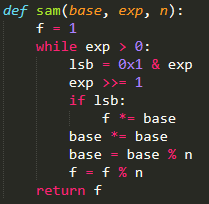
\includegraphics[width=0.345\linewidth]{images/SAM.png}
	\caption{Improved version of Square And Multiply}
	\label{fig:sam}
\end{figure}

%----------------------------------------------------------------------------------------
%	SECTION 5
%----------------------------------------------------------------------------------------

\section{Conclusion}

In this homework, as a difference with respect to the AES implementation, the code is based mainly on existent libraries, with the exception of few functions, whose implementation is based on pseudocode of already known algorithms, with small improvements in order to speed up the computations. The bigger improvement is the introduction of the modulo reduction on every computation of SAM, without it the proposed implementation didn't work as the result grew too much and it remained stuck after some iterations. As expected, also in this case the work is slower than the library implementation, with the exception of the key generation phase, which needs much more digging to reach the real cause of its larger throughput.

%----------------------------------------------------------------------------------------
%	BIBLIOGRAPHY
%----------------------------------------------------------------------------------------

\bibliographystyle{abbrv}

\bibliography{biblio}

%----------------------------------------------------------------------------------------


\end{document}